\documentclass[10pt]{article}
\PassOptionsToPackage{table}{xcolor}
\usepackage{tmlr}
% Camera-ready: \usepackage[accepted]{tmlr}.  De-anonymised preprint: \usepackage[preprint]{tmlr}.

%%%%% NEW MATH DEFINITIONS %%%%%

\usepackage{amsmath,amsfonts,bm}

% Mark sections of captions for referring to divisions of figures
\newcommand{\figleft}{{\em (Left)}}
\newcommand{\figcenter}{{\em (Center)}}
\newcommand{\figright}{{\em (Right)}}
\newcommand{\figtop}{{\em (Top)}}
\newcommand{\figbottom}{{\em (Bottom)}}
\newcommand{\captiona}{{\em (a)}}
\newcommand{\captionb}{{\em (b)}}
\newcommand{\captionc}{{\em (c)}}
\newcommand{\captiond}{{\em (d)}}

% Highlight a newly defined term
\newcommand{\newterm}[1]{{\bf #1}}


% Figure reference, lower-case.
\def\figref#1{figure~\ref{#1}}
% Figure reference, capital. For start of sentence
\def\Figref#1{Figure~\ref{#1}}
\def\twofigref#1#2{figures \ref{#1} and \ref{#2}}
\def\quadfigref#1#2#3#4{figures \ref{#1}, \ref{#2}, \ref{#3} and \ref{#4}}
% Section reference, lower-case.
\def\secref#1{section~\ref{#1}}
% Section reference, capital.
\def\Secref#1{Section~\ref{#1}}
% Reference to two sections.
\def\twosecrefs#1#2{sections \ref{#1} and \ref{#2}}
% Reference to three sections.
\def\secrefs#1#2#3{sections \ref{#1}, \ref{#2} and \ref{#3}}
% Reference to an equation, lower-case.
\def\eqref#1{equation~\ref{#1}}
% Reference to an equation, upper case
\def\Eqref#1{Equation~\ref{#1}}
% A raw reference to an equation---avoid using if possible
\def\plaineqref#1{\ref{#1}}
% Reference to a chapter, lower-case.
\def\chapref#1{chapter~\ref{#1}}
% Reference to an equation, upper case.
\def\Chapref#1{Chapter~\ref{#1}}
% Reference to a range of chapters
\def\rangechapref#1#2{chapters\ref{#1}--\ref{#2}}
% Reference to an algorithm, lower-case.
\def\algref#1{algorithm~\ref{#1}}
% Reference to an algorithm, upper case.
\def\Algref#1{Algorithm~\ref{#1}}
\def\twoalgref#1#2{algorithms \ref{#1} and \ref{#2}}
\def\Twoalgref#1#2{Algorithms \ref{#1} and \ref{#2}}
% Reference to a part, lower case
\def\partref#1{part~\ref{#1}}
% Reference to a part, upper case
\def\Partref#1{Part~\ref{#1}}
\def\twopartref#1#2{parts \ref{#1} and \ref{#2}}

\def\ceil#1{\lceil #1 \rceil}
\def\floor#1{\lfloor #1 \rfloor}
\def\1{\bm{1}}
\newcommand{\train}{\mathcal{D}}
\newcommand{\valid}{\mathcal{D_{\mathrm{valid}}}}
\newcommand{\test}{\mathcal{D_{\mathrm{test}}}}

\def\eps{{\epsilon}}


% Random variables
\def\reta{{\textnormal{$\eta$}}}
\def\ra{{\textnormal{a}}}
\def\rb{{\textnormal{b}}}
\def\rc{{\textnormal{c}}}
\def\rd{{\textnormal{d}}}
\def\re{{\textnormal{e}}}
\def\rf{{\textnormal{f}}}
\def\rg{{\textnormal{g}}}
\def\rh{{\textnormal{h}}}
\def\ri{{\textnormal{i}}}
\def\rj{{\textnormal{j}}}
\def\rk{{\textnormal{k}}}
\def\rl{{\textnormal{l}}}
% rm is already a command, just don't name any random variables m
\def\rn{{\textnormal{n}}}
\def\ro{{\textnormal{o}}}
\def\rp{{\textnormal{p}}}
\def\rq{{\textnormal{q}}}
\def\rr{{\textnormal{r}}}
\def\rs{{\textnormal{s}}}
\def\rt{{\textnormal{t}}}
\def\ru{{\textnormal{u}}}
\def\rv{{\textnormal{v}}}
\def\rw{{\textnormal{w}}}
\def\rx{{\textnormal{x}}}
\def\ry{{\textnormal{y}}}
\def\rz{{\textnormal{z}}}

% Random vectors
\def\rvepsilon{{\mathbf{\epsilon}}}
\def\rvtheta{{\mathbf{\theta}}}
\def\rva{{\mathbf{a}}}
\def\rvb{{\mathbf{b}}}
\def\rvc{{\mathbf{c}}}
\def\rvd{{\mathbf{d}}}
\def\rve{{\mathbf{e}}}
\def\rvf{{\mathbf{f}}}
\def\rvg{{\mathbf{g}}}
\def\rvh{{\mathbf{h}}}
\def\rvu{{\mathbf{i}}}
\def\rvj{{\mathbf{j}}}
\def\rvk{{\mathbf{k}}}
\def\rvl{{\mathbf{l}}}
\def\rvm{{\mathbf{m}}}
\def\rvn{{\mathbf{n}}}
\def\rvo{{\mathbf{o}}}
\def\rvp{{\mathbf{p}}}
\def\rvq{{\mathbf{q}}}
\def\rvr{{\mathbf{r}}}
\def\rvs{{\mathbf{s}}}
\def\rvt{{\mathbf{t}}}
\def\rvu{{\mathbf{u}}}
\def\rvv{{\mathbf{v}}}
\def\rvw{{\mathbf{w}}}
\def\rvx{{\mathbf{x}}}
\def\rvy{{\mathbf{y}}}
\def\rvz{{\mathbf{z}}}

% Elements of random vectors
\def\erva{{\textnormal{a}}}
\def\ervb{{\textnormal{b}}}
\def\ervc{{\textnormal{c}}}
\def\ervd{{\textnormal{d}}}
\def\erve{{\textnormal{e}}}
\def\ervf{{\textnormal{f}}}
\def\ervg{{\textnormal{g}}}
\def\ervh{{\textnormal{h}}}
\def\ervi{{\textnormal{i}}}
\def\ervj{{\textnormal{j}}}
\def\ervk{{\textnormal{k}}}
\def\ervl{{\textnormal{l}}}
\def\ervm{{\textnormal{m}}}
\def\ervn{{\textnormal{n}}}
\def\ervo{{\textnormal{o}}}
\def\ervp{{\textnormal{p}}}
\def\ervq{{\textnormal{q}}}
\def\ervr{{\textnormal{r}}}
\def\ervs{{\textnormal{s}}}
\def\ervt{{\textnormal{t}}}
\def\ervu{{\textnormal{u}}}
\def\ervv{{\textnormal{v}}}
\def\ervw{{\textnormal{w}}}
\def\ervx{{\textnormal{x}}}
\def\ervy{{\textnormal{y}}}
\def\ervz{{\textnormal{z}}}

% Random matrices
\def\rmA{{\mathbf{A}}}
\def\rmB{{\mathbf{B}}}
\def\rmC{{\mathbf{C}}}
\def\rmD{{\mathbf{D}}}
\def\rmE{{\mathbf{E}}}
\def\rmF{{\mathbf{F}}}
\def\rmG{{\mathbf{G}}}
\def\rmH{{\mathbf{H}}}
\def\rmI{{\mathbf{I}}}
\def\rmJ{{\mathbf{J}}}
\def\rmK{{\mathbf{K}}}
\def\rmL{{\mathbf{L}}}
\def\rmM{{\mathbf{M}}}
\def\rmN{{\mathbf{N}}}
\def\rmO{{\mathbf{O}}}
\def\rmP{{\mathbf{P}}}
\def\rmQ{{\mathbf{Q}}}
\def\rmR{{\mathbf{R}}}
\def\rmS{{\mathbf{S}}}
\def\rmT{{\mathbf{T}}}
\def\rmU{{\mathbf{U}}}
\def\rmV{{\mathbf{V}}}
\def\rmW{{\mathbf{W}}}
\def\rmX{{\mathbf{X}}}
\def\rmY{{\mathbf{Y}}}
\def\rmZ{{\mathbf{Z}}}

% Elements of random matrices
\def\ermA{{\textnormal{A}}}
\def\ermB{{\textnormal{B}}}
\def\ermC{{\textnormal{C}}}
\def\ermD{{\textnormal{D}}}
\def\ermE{{\textnormal{E}}}
\def\ermF{{\textnormal{F}}}
\def\ermG{{\textnormal{G}}}
\def\ermH{{\textnormal{H}}}
\def\ermI{{\textnormal{I}}}
\def\ermJ{{\textnormal{J}}}
\def\ermK{{\textnormal{K}}}
\def\ermL{{\textnormal{L}}}
\def\ermM{{\textnormal{M}}}
\def\ermN{{\textnormal{N}}}
\def\ermO{{\textnormal{O}}}
\def\ermP{{\textnormal{P}}}
\def\ermQ{{\textnormal{Q}}}
\def\ermR{{\textnormal{R}}}
\def\ermS{{\textnormal{S}}}
\def\ermT{{\textnormal{T}}}
\def\ermU{{\textnormal{U}}}
\def\ermV{{\textnormal{V}}}
\def\ermW{{\textnormal{W}}}
\def\ermX{{\textnormal{X}}}
\def\ermY{{\textnormal{Y}}}
\def\ermZ{{\textnormal{Z}}}

% Vectors
\def\vzero{{\bm{0}}}
\def\vone{{\bm{1}}}
\def\vmu{{\bm{\mu}}}
\def\vtheta{{\bm{\theta}}}
\def\va{{\bm{a}}}
\def\vb{{\bm{b}}}
\def\vc{{\bm{c}}}
\def\vd{{\bm{d}}}
\def\ve{{\bm{e}}}
\def\vf{{\bm{f}}}
\def\vg{{\bm{g}}}
\def\vh{{\bm{h}}}
\def\vi{{\bm{i}}}
\def\vj{{\bm{j}}}
\def\vk{{\bm{k}}}
\def\vl{{\bm{l}}}
\def\vm{{\bm{m}}}
\def\vn{{\bm{n}}}
\def\vo{{\bm{o}}}
\def\vp{{\bm{p}}}
\def\vq{{\bm{q}}}
\def\vr{{\bm{r}}}
\def\vs{{\bm{s}}}
\def\vt{{\bm{t}}}
\def\vu{{\bm{u}}}
\def\vv{{\bm{v}}}
\def\vw{{\bm{w}}}
\def\vx{{\bm{x}}}
\def\vy{{\bm{y}}}
\def\vz{{\bm{z}}}

% Elements of vectors
\def\evalpha{{\alpha}}
\def\evbeta{{\beta}}
\def\evepsilon{{\epsilon}}
\def\evlambda{{\lambda}}
\def\evomega{{\omega}}
\def\evmu{{\mu}}
\def\evpsi{{\psi}}
\def\evsigma{{\sigma}}
\def\evtheta{{\theta}}
\def\eva{{a}}
\def\evb{{b}}
\def\evc{{c}}
\def\evd{{d}}
\def\eve{{e}}
\def\evf{{f}}
\def\evg{{g}}
\def\evh{{h}}
\def\evi{{i}}
\def\evj{{j}}
\def\evk{{k}}
\def\evl{{l}}
\def\evm{{m}}
\def\evn{{n}}
\def\evo{{o}}
\def\evp{{p}}
\def\evq{{q}}
\def\evr{{r}}
\def\evs{{s}}
\def\evt{{t}}
\def\evu{{u}}
\def\evv{{v}}
\def\evw{{w}}
\def\evx{{x}}
\def\evy{{y}}
\def\evz{{z}}

% Matrix
\def\mA{{\bm{A}}}
\def\mB{{\bm{B}}}
\def\mC{{\bm{C}}}
\def\mD{{\bm{D}}}
\def\mE{{\bm{E}}}
\def\mF{{\bm{F}}}
\def\mG{{\bm{G}}}
\def\mH{{\bm{H}}}
\def\mI{{\bm{I}}}
\def\mJ{{\bm{J}}}
\def\mK{{\bm{K}}}
\def\mL{{\bm{L}}}
\def\mM{{\bm{M}}}
\def\mN{{\bm{N}}}
\def\mO{{\bm{O}}}
\def\mP{{\bm{P}}}
\def\mQ{{\bm{Q}}}
\def\mR{{\bm{R}}}
\def\mS{{\bm{S}}}
\def\mT{{\bm{T}}}
\def\mU{{\bm{U}}}
\def\mV{{\bm{V}}}
\def\mW{{\bm{W}}}
\def\mX{{\bm{X}}}
\def\mY{{\bm{Y}}}
\def\mZ{{\bm{Z}}}
\def\mBeta{{\bm{\beta}}}
\def\mPhi{{\bm{\Phi}}}
\def\mLambda{{\bm{\Lambda}}}
\def\mSigma{{\bm{\Sigma}}}

% Tensor
\DeclareMathAlphabet{\mathsfit}{\encodingdefault}{\sfdefault}{m}{sl}
\SetMathAlphabet{\mathsfit}{bold}{\encodingdefault}{\sfdefault}{bx}{n}
\newcommand{\tens}[1]{\bm{\mathsfit{#1}}}
\def\tA{{\tens{A}}}
\def\tB{{\tens{B}}}
\def\tC{{\tens{C}}}
\def\tD{{\tens{D}}}
\def\tE{{\tens{E}}}
\def\tF{{\tens{F}}}
\def\tG{{\tens{G}}}
\def\tH{{\tens{H}}}
\def\tI{{\tens{I}}}
\def\tJ{{\tens{J}}}
\def\tK{{\tens{K}}}
\def\tL{{\tens{L}}}
\def\tM{{\tens{M}}}
\def\tN{{\tens{N}}}
\def\tO{{\tens{O}}}
\def\tP{{\tens{P}}}
\def\tQ{{\tens{Q}}}
\def\tR{{\tens{R}}}
\def\tS{{\tens{S}}}
\def\tT{{\tens{T}}}
\def\tU{{\tens{U}}}
\def\tV{{\tens{V}}}
\def\tW{{\tens{W}}}
\def\tX{{\tens{X}}}
\def\tY{{\tens{Y}}}
\def\tZ{{\tens{Z}}}


% Graph
\def\gA{{\mathcal{A}}}
\def\gB{{\mathcal{B}}}
\def\gC{{\mathcal{C}}}
\def\gD{{\mathcal{D}}}
\def\gE{{\mathcal{E}}}
\def\gF{{\mathcal{F}}}
\def\gG{{\mathcal{G}}}
\def\gH{{\mathcal{H}}}
\def\gI{{\mathcal{I}}}
\def\gJ{{\mathcal{J}}}
\def\gK{{\mathcal{K}}}
\def\gL{{\mathcal{L}}}
\def\gM{{\mathcal{M}}}
\def\gN{{\mathcal{N}}}
\def\gO{{\mathcal{O}}}
\def\gP{{\mathcal{P}}}
\def\gQ{{\mathcal{Q}}}
\def\gR{{\mathcal{R}}}
\def\gS{{\mathcal{S}}}
\def\gT{{\mathcal{T}}}
\def\gU{{\mathcal{U}}}
\def\gV{{\mathcal{V}}}
\def\gW{{\mathcal{W}}}
\def\gX{{\mathcal{X}}}
\def\gY{{\mathcal{Y}}}
\def\gZ{{\mathcal{Z}}}

% Sets
\def\sA{{\mathbb{A}}}
\def\sB{{\mathbb{B}}}
\def\sC{{\mathbb{C}}}
\def\sD{{\mathbb{D}}}
% Don't use a set called E, because this would be the same as our symbol
% for expectation.
\def\sF{{\mathbb{F}}}
\def\sG{{\mathbb{G}}}
\def\sH{{\mathbb{H}}}
\def\sI{{\mathbb{I}}}
\def\sJ{{\mathbb{J}}}
\def\sK{{\mathbb{K}}}
\def\sL{{\mathbb{L}}}
\def\sM{{\mathbb{M}}}
\def\sN{{\mathbb{N}}}
\def\sO{{\mathbb{O}}}
\def\sP{{\mathbb{P}}}
\def\sQ{{\mathbb{Q}}}
\def\sR{{\mathbb{R}}}
\def\sS{{\mathbb{S}}}
\def\sT{{\mathbb{T}}}
\def\sU{{\mathbb{U}}}
\def\sV{{\mathbb{V}}}
\def\sW{{\mathbb{W}}}
\def\sX{{\mathbb{X}}}
\def\sY{{\mathbb{Y}}}
\def\sZ{{\mathbb{Z}}}

% Entries of a matrix
\def\emLambda{{\Lambda}}
\def\emA{{A}}
\def\emB{{B}}
\def\emC{{C}}
\def\emD{{D}}
\def\emE{{E}}
\def\emF{{F}}
\def\emG{{G}}
\def\emH{{H}}
\def\emI{{I}}
\def\emJ{{J}}
\def\emK{{K}}
\def\emL{{L}}
\def\emM{{M}}
\def\emN{{N}}
\def\emO{{O}}
\def\emP{{P}}
\def\emQ{{Q}}
\def\emR{{R}}
\def\emS{{S}}
\def\emT{{T}}
\def\emU{{U}}
\def\emV{{V}}
\def\emW{{W}}
\def\emX{{X}}
\def\emY{{Y}}
\def\emZ{{Z}}
\def\emSigma{{\Sigma}}

% entries of a tensor
% Same font as tensor, without \bm wrapper
\newcommand{\etens}[1]{\mathsfit{#1}}
\def\etLambda{{\etens{\Lambda}}}
\def\etA{{\etens{A}}}
\def\etB{{\etens{B}}}
\def\etC{{\etens{C}}}
\def\etD{{\etens{D}}}
\def\etE{{\etens{E}}}
\def\etF{{\etens{F}}}
\def\etG{{\etens{G}}}
\def\etH{{\etens{H}}}
\def\etI{{\etens{I}}}
\def\etJ{{\etens{J}}}
\def\etK{{\etens{K}}}
\def\etL{{\etens{L}}}
\def\etM{{\etens{M}}}
\def\etN{{\etens{N}}}
\def\etO{{\etens{O}}}
\def\etP{{\etens{P}}}
\def\etQ{{\etens{Q}}}
\def\etR{{\etens{R}}}
\def\etS{{\etens{S}}}
\def\etT{{\etens{T}}}
\def\etU{{\etens{U}}}
\def\etV{{\etens{V}}}
\def\etW{{\etens{W}}}
\def\etX{{\etens{X}}}
\def\etY{{\etens{Y}}}
\def\etZ{{\etens{Z}}}

% The true underlying data generating distribution
\newcommand{\pdata}{p_{\rm{data}}}
% The empirical distribution defined by the training set
\newcommand{\ptrain}{\hat{p}_{\rm{data}}}
\newcommand{\Ptrain}{\hat{P}_{\rm{data}}}
% The model distribution
\newcommand{\pmodel}{p_{\rm{model}}}
\newcommand{\Pmodel}{P_{\rm{model}}}
\newcommand{\ptildemodel}{\tilde{p}_{\rm{model}}}
% Stochastic autoencoder distributions
\newcommand{\pencode}{p_{\rm{encoder}}}
\newcommand{\pdecode}{p_{\rm{decoder}}}
\newcommand{\precons}{p_{\rm{reconstruct}}}

\newcommand{\laplace}{\mathrm{Laplace}} % Laplace distribution

\newcommand{\E}{\mathbb{E}}
\newcommand{\Ls}{\mathcal{L}}
\newcommand{\R}{\mathbb{R}}
\newcommand{\emp}{\tilde{p}}
\newcommand{\lr}{\alpha}
\newcommand{\reg}{\lambda}
\newcommand{\rect}{\mathrm{rectifier}}
\newcommand{\softmax}{\mathrm{softmax}}
\newcommand{\sigmoid}{\sigma}
\newcommand{\softplus}{\zeta}
\newcommand{\KL}{D_{\mathrm{KL}}}
\newcommand{\Var}{\mathrm{Var}}
\newcommand{\standarderror}{\mathrm{SE}}
\newcommand{\Cov}{\mathrm{Cov}}
% Wolfram Mathworld says $L^2$ is for function spaces and $\ell^2$ is for vectors
% But then they seem to use $L^2$ for vectors throughout the site, and so does
% wikipedia.
\newcommand{\normlzero}{L^0}
\newcommand{\normlone}{L^1}
\newcommand{\normltwo}{L^2}
\newcommand{\normlp}{L^p}
\newcommand{\normmax}{L^\infty}

\newcommand{\parents}{Pa} % See usage in notation.tex. Chosen to match Daphne's book.

\DeclareMathOperator*{\argmax}{arg\,max}
\DeclareMathOperator*{\argmin}{arg\,min}

\DeclareMathOperator{\sign}{sign}
\DeclareMathOperator{\Tr}{Tr}
\let\ab\allowbreak


\usepackage{hyperref}
\usepackage{url}
\usepackage{amsmath,amssymb,amsthm,mathtools,bm}
\usepackage{xcolor}
\usepackage{booktabs,multirow,graphicx}
\usepackage{caption}
\usepackage{placeins}
\usepackage{tikz}
\usetikzlibrary{arrows.meta,positioning,fit,calc}

\definecolor{oursbg}{RGB}{232,240,251}  % light band for our models in result tables
\renewcommand{\arraystretch}{1.12}
\renewcommand{\topfraction}{0.9}\renewcommand{\bottomfraction}{0.8}
\renewcommand{\textfraction}{0.07}\renewcommand{\floatpagefraction}{0.7}

\newtheorem{theorem}{Theorem}
\newtheorem{proposition}[theorem]{Proposition}
\newtheorem{lemma}[theorem]{Lemma}
\newtheorem{corollary}[theorem]{Corollary}
\theoremstyle{remark}
\newtheorem{remark}[theorem]{Remark}

\newcommand{\dd}{\,\mathrm{d}}
\newcommand{\codename}{supplementary code}  % how this version refers to its code

\title{Exact Phase-Type Point Processes for\\
Certified Measurement and Prediction of Event Streams}

% Anonymous for review: authors are hidden unless the [accepted] or [preprint] option is used.
\author{\name Sayak Dutta \email sayakdutta1002@gmail.com}

\def\month{MM}
\def\year{YYYY}
\def\openreview{\url{https://openreview.net/forum?id=XXXX}}

\newcommand{\rhoPooled}{0.87}
\newcommand{\relaxPooled}{12}
\newcommand{\placeboCpi}{8.5}
\newcommand{\placeboNfp}{6.7}
\newcommand{\placeboPpi}{4.0}
\newcommand{\placeboFomc}{3.9}
\newcommand{\placeboRetail}{1.9}
\newcommand{\nPassPlacebo}{5}
\newcommand{\nKinds}{11}
\newcommand{\tDirMed}{1.1}
\newcommand{\tEchoLo}{16}\newcommand{\tEchoHi}{137}
\newcommand{\tNinetyLo}{5}\newcommand{\tNinetyHi}{11}
\newcommand{\ksMax}{0.044}
\newcommand{\edLo}{26}\newcommand{\edHi}{55}
\newcommand{\gapMaxPooled}{0.0054}
\newcommand{\nWindows}{732}
\newcommand{\nEventsScored}{7.3}
\newcommand{\nEventsAll}{8.4}
\newcommand{\nNewsWindows}{430}\newcommand{\nPlaceboWindows}{302}
\newcommand{\vOnePlacebo}{169}
\newcommand{\vOneKSmax}{0.58}
\newcommand{\vTwoPlacebo}{18.6}
\newcommand{\eptNoBackbone}{2.84}
\newcommand{\lOneSelected}{0.8}
\newcommand{\trackCwins}{5}\newcommand{\trackCdone}{5}
\newcommand{\trackCmarginLo}{0.23}\newcommand{\trackCmarginHi}{0.41}
\newcommand{\driftCorrOursOne}{0.17}\newcommand{\driftCorrBaseOne}{0.06}
\newcommand{\bestActivityModel}{event-study OLS}
\newcommand{\nTestReleases}{163}
\newcommand{\eptxSeeds}{Amazon three; Retweet two; Taxi five; Taobao three; StackOverflow three}
\newcommand{\rhoByYear}{0.91, 0.89, 0.85, 0.86, 0.85}


\newcommand{\pubsrc}{\citealp{chang2025deep,boyd2025hyper}}  % source of the published benchmark numbers
\begin{document}
\maketitle

\begin{abstract}
Temporal point processes are used both to \emph{measure} market mechanisms, for example how fast
prices absorb news and how much of the reaction is the market responding to itself, and to
\emph{predict} the next event. We show that one algebraic object, the phase-type (Erlang-chain)
state space, serves both purposes with exact likelihoods. For measurement, we build a multiscale
phase-type Hawkes process whose parameters all enter linearly. Its log-likelihood is concave, and
we compute the global maximum together with a Fenchel duality-gap certificate. A Markov embedding
gives the response to an exogenous shock, echoes included, in closed form, and this response is
stable if and only if the spectral radius of the branching matrix is below one. Applied to six
markets around 670 scheduled macroeconomic releases (2022--2026) with a built-in placebo test, the
model shows that the direct reaction to CPI, payrolls, PPI and the FOMC statement is absorbed in
about a second, while the market's own echoes stretch half of the response to
\tEchoLo--\tEchoHi{}\,s. For prediction, we introduce EPT-X, a neural point process that adds a
history-dependent mixture-of-Erlang renewal channel to a linear Hawkes backbone. Its intensity
and compensator remain in closed form, so it is trained and evaluated on the exact likelihood.
EPT-X has the best test likelihood on all five LOBSTER order-book streams against six classical
estimators and seven neural baselines, improves the best published result on Retweet by more
than 0.6~nats per event, is within one standard deviation of it on Taobao and StackOverflow, and
trails the state-space model S2P2 on Taxi and Amazon. We also find that a widely used
IntensityFree implementation clamps short inter-event times before scoring, which overstates its
likelihood on streams with many short gaps.

\end{abstract}

\section{Introduction}\label{sec:intro}

Event streams in markets---price changes, order-book messages, trades---are modelled with
temporal point processes for two different purposes. Econometricians use Hawkes processes
\citep{hawkes1971spectra} to \emph{measure} mechanisms: the branching structure separates
exogenous, news-driven events from endogenous ones triggered by earlier events, and the
fitted kernels quantify how fast information is absorbed
\citep{hardiman2013critical,filimonov2012quantifying,rambaldi2015modeling}. Machine-learning
work uses neural temporal point processes to \emph{predict} the next event and is judged by
held-out likelihood on shared benchmarks
\citep{du2016recurrent,mei2017neural,zuo2020transformer,shchur2020intensity,xue2024easytpp,chang2025deep}.
The two communities rarely meet, and each inherits a weakness. Measurement relies on
non-convex fits whose optimality is unknown and on summaries---such as the ``half-life''
$\ln2/\beta$ of a news kernel---that ignore the echoes the news triggers. On the prediction
side, most intensity-based neural models estimate the compensator $\int\lambda$ by Monte Carlo
\citep{mei2017neural,zuo2020transformer,yang2022transformer,chang2025deep}, so that reported
likelihoods carry sampling error; models with an exact likelihood exist---through a monotone
network for the cumulative hazard \citep{omi2019fully} or a mixture density for the next gap
\citep{shchur2020intensity}---but give up the Hawkes structure that makes a model interpretable
\citep{shchur2021neural}. As we show, reported likelihoods are also sensitive to implementation
details.

We argue that one algebraic object serves both purposes exactly: the \emph{phase-type
state space}, in which every kernel is a nonnegative combination of Erlang densities on a
logarithmic grid of time scales. Between events such a state evolves by an explicit matrix
exponential, so intensities and compensators are available in closed form, and the class is
dense in the densities on $\R_+$.

\paragraph{Contributions.}
\begin{enumerate}
\item \textbf{Certified measurement (MSX).} A multiscale phase-type Hawkes process with
exogenous, marked news kernels in which all parameters enter linearly. The log-likelihood is
concave; we compute the global maximum with accelerated EM and a barrier-Newton polish and
return a Fenchel duality gap that certifies optimality (Proposition~\ref{prop:gap}).
\item \textbf{Echo-corrected responses in closed form.} A Markov embedding turns the mean
response to a shock into $C e^{\mathcal At}\bm z_0$; it is stable if and only if
$\rho(G)<1$ for the branching matrix $G$ (Theorem~\ref{thm:stab}), and yields absorption
quantiles, echo amplification and price-discovery curves without simulation.
\item \textbf{Exact neural prediction (EPT-X).} A neural point process whose latent state is
phase-type, with a linear Hawkes backbone and a history-conditioned \emph{defective
hyper-Erlang renewal channel} superposed as a competing risk. The compensator stays exact,
the model nests the Hawkes backbone, and the renewal channel is universal for the conditional
gap law (Proposition~\ref{prop:eptx}).
\item \textbf{Benchmarks and a benchmark correction.} EPT-X is best on all five LOBSTER
order-book streams and on Retweet, and statistically tied with the best published model on
Taobao and StackOverflow. We find that a widely used IntensityFree implementation clamps
inter-event times at $10^{-5}$\,s before scoring; re-scored on the observed gaps, its lead on
two order-book streams disappears.
\item \textbf{Application.} On six markets around 670 scheduled releases (2022--2026), with a
placebo test built into the likelihood, we find that the direct reaction to CPI, payrolls,
PPI and the FOMC is absorbed in about a second while echoes stretch half of the response to
\tEchoLo--\tEchoHi{}\,s and ninety percent to \tNinetyLo--\tNinetyHi{} minutes.
\end{enumerate}
Linear-in-parameters kernel dictionaries \citep{bacry2015hawkes}, EM for Hawkes processes
\citep{veen2008estimation,zhou2013learning}, Erlang-chain embeddings and exact-likelihood neural
point processes \citep{omi2019fully,shchur2020intensity} are known individually; our contribution
is their combination into certified, closed-form measurement and into an exact-likelihood neural
model that nests the linear Hawkes process, together with the evidence that both work.

\section{Related work}\label{sec:related}

\paragraph{Hawkes estimation.} Exponential and sum-of-exponential kernels are fitted by
maximum likelihood \citep{bacry2015hawkes}, for instance with the \texttt{tick} library
\citep{bacry2018tick}; alternatives include EM algorithms that exploit the branching structure
\citep{veen2008estimation}, ADM4 with low-rank and sparse penalties
\citep{zhou2013learning}, the conditional-law (Wiener--Hopf) method \citep{bacry2016estimation},
cumulant matching \citep{achab2017uncovering} and INAR approximations
\citep{kirchner2017estimation}. None of these returns a certificate of global optimality for
multiscale kernels with humps, and seasonality mis-specification is known to bias branching
ratios upward \citep{filimonov2015apparent,omi2017hawkes}.

\paragraph{News in Hawkes models.} \citet{rambaldi2015modeling} add an exogenous kernel for
macroeconomic announcements to an FX Hawkes model; \citet{andersen2003micro} document the
price impact of announcement surprises. Absorption speed is typically read off the
exogenous kernel alone. We give the echo-corrected response in closed form and test the news
kernels against matched placebo windows inside the likelihood.

\paragraph{Neural temporal point processes.} See \citet{shchur2021neural} for a review. RMTPP
\citep{du2016recurrent} uses an exponential intensity between events, whose integral is closed
form. NHP \citep{mei2017neural}, SAHP \citep{zhang2020self}, THP \citep{zuo2020transformer},
AttNHP \citep{yang2022transformer} and the state-space S2P2 \citep{chang2025deep} parameterise
the intensity with recurrent, attention or state-space encoders and estimate the compensator by
Monte Carlo or quadrature. FullyNN \citep{omi2019fully} models the cumulative hazard with a
monotone network and IntensityFree \citep{shchur2020intensity} the next-gap density with a
log-normal mixture; both have exact likelihoods but no Hawkes structure. Recent work explores Mamba-style encoders
\citep{gao2024mamba} and interpretable latent Hawkes dynamics \citep{boyd2025hyper}.
EasyTPP \citep{xue2024easytpp} provides shared implementations, and
\citet{bosser2023predictive} study the predictive accuracy of neural TPPs. EPT-X differs in
that its intensity between events is a read-out of an explicitly solvable phase-type system
with bounded closed-form hazard terms, plus a renewal channel whose survival function is a closed-form mixture of Erlang
survivals---so the likelihood we train and report is exact---and in that its backbone is the
linear Hawkes process itself, so the fitted model retains branching ratios and excitation
kernels that can be read off.

\paragraph{Phase-type distributions.} Mixtures of Erlang distributions are dense in the
distributions on $(0,\infty)$ \citep{tijms1994stochastic,lee2010modeling}; we use this fact
for the renewal channel and the Erlang-chain recursion for all states.

\section{Phase-type state spaces}\label{sec:phasetype}

\paragraph{A dictionary of Erlang densities.} Fix a set of rates $\beta_1,\dots,\beta_K>0$ on a
logarithmic grid, so that each rate corresponds to a time scale $1/\beta_k$, and an Erlang order
$R\ge1$. For $k=1,\dots,K$ and $r=0,\dots,R-1$ we define the basis densities
\begin{equation}\label{eq:basis}
g_{kr}(t)=\beta_k\,\frac{(\beta_k t)^r}{r!}\,e^{-\beta_k t},\qquad t\ge0 .
\end{equation}
Each $g_{kr}$ is the density of a gamma (Erlang) distribution with shape $r+1$ and rate
$\beta_k$, so $\int_0^\infty g_{kr}(t)\,\mathrm{d}t=1$ and its mean is $(r+1)/\beta_k$. A kernel is a
nonnegative combination
\begin{equation}\label{eq:kernel}
\phi(t)=\sum_{k=1}^{K}\sum_{r=0}^{R-1}a_{kr}\,g_{kr}(t),\qquad a_{kr}\ge0 .
\end{equation}
Because each basis density integrates to one, the total mass of the kernel, which is its
branching ratio, is simply $\sum_{k,r}a_{kr}$. With $R=1$ the dictionary contains only
exponentials, and mixtures of exponentials can approximate any completely monotone kernel,
power laws included (Bernstein's theorem). Orders $r\ge1$ add kernels that start at zero and peak
later, which describe delayed reactions. More generally, phase-type densities are dense in the set
of densities on $\R_+$.

\paragraph{Exact recursion.} Every state in this paper is built from such Erlang chains: the
Hawkes excitation, the response to news, the neural latent state of EPT and the renewal channel of
EPT-X. For all of them, the evolution between two events and its integral are available in closed
form. The following lemma gives the formulas for one source and one rate.

\begin{lemma}[Erlang-chain recursion]\label{lem:recursion}
Let $t_1<t_2<\dots$ be the event times of one source, let $\beta>0$ be one rate of the
dictionary, and define the chain of states
\[
s_r(t)=\sum_{n:\,t_n<t} g_r(t-t_n),\qquad r=0,\dots,R-1,
\]
where $g_r$ is the basis density~(\ref{eq:basis}) with rate $\beta$. Write
$\bm s=(s_0,\dots,s_{R-1})^\top$, let $I$ be the $R\times R$ identity and let $B$ be the
$R\times R$ down-shift matrix ($B_{r,r-1}=1$ and all other entries zero).
\begin{enumerate}
\item Between events, $\dot{\bm s}=\beta(B-I)\,\bm s$; at an event, $s_0$ increases by $\beta$.
\item For a gap $\Delta\ge0$ with no event in $(t,t+\Delta)$, let $y=\beta\Delta$ and
$w_j=e^{-y}y^j/j!$. Then
\[
s_r(t+\Delta)=\sum_{j=0}^{r}w_j\,s_{r-j}(t),\qquad
\int_t^{t+\Delta}s_r(u)\,\mathrm{d}u=\frac{1}{\beta}\sum_{j=0}^{r}P(j+1,y)\,s_{r-j}(t),
\]
where $P(a,y)$ is the regularised lower incomplete gamma function.
\end{enumerate}
\end{lemma}

\begin{proof}
\emph{Step 1 (dynamics).} Differentiating~(\ref{eq:basis}) gives
\[
\frac{\mathrm{d}}{\mathrm{d}t}g_0(t)=-\beta\,g_0(t),\qquad
\frac{\mathrm{d}}{\mathrm{d}t}g_r(t)=\beta\bigl(g_{r-1}(t)-g_r(t)\bigr)\quad(r\ge1).
\]
Summing over past events gives $\dot s_0=-\beta s_0$ and $\dot s_r=\beta(s_{r-1}-s_r)$, which is
$\dot{\bm s}=\beta(B-I)\bm s$. Since $g_r(0)=\beta\,\mathbb{1}[r=0]$, a new event adds $\beta$ to
$s_0$ and leaves the other states unchanged.

\emph{Step 2 (evolution over a gap).} The solution is $\bm s(t+\Delta)=e^{\beta(B-I)\Delta}\bm s(t)$.
The matrices $B$ and $I$ commute and $B^R=0$, so
\[
e^{\beta(B-I)\Delta}=e^{-y}\,e^{yB}=e^{-y}\sum_{j=0}^{R-1}\frac{y^j}{j!}B^j .
\]
Because $B^j$ shifts a vector down by $j$ places, component $r$ of $e^{\beta(B-I)\Delta}\bm s(t)$
is $\sum_{j\le r}w_j s_{r-j}(t)$.

\emph{Step 3 (integral over a gap).} Integrating the weights over the gap,
\[
\int_0^{\Delta}e^{-\beta u}\frac{(\beta u)^j}{j!}\,\mathrm{d}u=\frac{1}{\beta}\,P(j+1,y),
\]
which gives the second formula.
\end{proof}

Evaluating a likelihood therefore costs $O(N d K R^2)$ operations for $N$ events in $d$
dimensions, and it involves no Monte Carlo or quadrature error.

\section{MSX: certified measurement with echo-corrected responses}\label{sec:msx}

\paragraph{Model.} Consider $d$ event dimensions observed in windows $w$ with likelihood
intervals $[t_0^w,t_1^w)$, and exogenous shocks $e$ (here: scheduled releases) at times
$\tau_e$ with type $c_e$ and nonnegative mark features $\bm z_e=(1,z_e^+,z_e^-)$, the
standardised surprise split by sign. The MSX intensity of dimension $i$ is
\begin{align}
\lambda_i(t)={}&\underbrace{c_{iw}+\textstyle\sum_{m}\eta_{im}h_m(\mathrm{tod}(t))}_{\text{baseline}}
+\underbrace{\sum_{j}\sum_{t_n^j<t}\sum_{k,r}a_{ijkr}\,g_{kr}(t-t_n^j)}_{\text{endogenous}}\nonumber\\
&+\underbrace{\sum_{e:\tau_e<t}\sum_{k,r,m}b_{i c_e k r m}\,z_{em}\,g^{\rm exo}_{kr}(t-\tau_e)}_{\text{exogenous (news)}}
+\underbrace{\sum_{e:\tau_e>t}\sum_{k}\alpha_{ic_ek}\,\beta^{\rm ant}_k e^{-\beta^{\rm ant}_k(\tau_e-t)}}_{\text{anticipation}},
\label{eq:intensity}
\end{align}
with per-window intercepts $c_{iw}$, periodic hat functions $h_m$ of local time of day, and
all parameters nonnegative. Writing $\bm x(t)\ge0$ for the stacked features,
$\lambda_i(t)=\bm x(t)^\top\bm\theta_i$, and the log-likelihood separates across targets,
\begin{equation}
\ell_i(\bm\theta_i)=\sum_{n:\,u_n=i}\log\big(\bm x(t_n)^\top\bm\theta_i\big)-\bm\Phi^\top\bm\theta_i,
\qquad \bm\Phi=\sum_w\int_{t_0^w}^{t_1^w}\bm x(t)\dd t,\label{eq:ll}
\end{equation}
where every entry of $\bm x(t_n)$ and $\bm\Phi$ follows from Lemma~\ref{lem:recursion}.

\paragraph{Concavity and a certificate.} Problem~\eqref{eq:ll} maximises a concave function
over the nonnegative orthant. Exposure-weighted $\ell_1$ penalties are linear,
$\bm\gamma^\top\bm\theta$, and are absorbed into $\bm\Phi$. We run the multiplicative EM map
$\theta_p\leftarrow\theta_p\,(\sum_n x_{np}/\lambda_n)/(\Phi_p+\gamma_p)$, accelerated by
SQUAREM \citep{varadhan2008simple}, and polish with a log-barrier Newton method.

\begin{proposition}[Duality-gap certificate]\label{prop:gap}
For any feasible $\bm\theta\ge0$ with intensities $\lambda_n=\bm x_n^\top\bm\theta>0$, let
$s=\max_p (X^\top\bm\lambda^{-1})_p/(\Phi_p+\gamma_p)$. Then
\[
\ell^\star-\ell(\bm\theta)\;\le\;N\log s+\big(\bm\theta^\top(\bm\Phi+\bm\gamma)-N\big),
\]
and both terms vanish at the optimum.
\end{proposition}
The proof (Appendix~\ref{app:proofs}) applies Fenchel's inequality $\log u\le vu-1-\log v$ to
each $\lambda_n$. Every fit reported here carries this certificate.

\paragraph{Markov embedding.} Stack the endogenous states into $\bm x$, let $F$ be the
block-diagonal Erlang-chain generator, $G_{\rm in}$ inject $\beta_k$ into phase $r=0$ of a
source, and $\Theta$ the endogenous weights. The \emph{mean} excess intensity caused by one
shock with exogenous states $\bm y$ ($\dot{\bm y}=F_e\bm y$, $\bm y(0)=\bm y_0$) solves
\begin{equation}
\dot{\bm z}=\mathcal A\bm z,\quad
\mathcal A=\begin{pmatrix}F+G_{\rm in}\Theta & G_{\rm in}\Theta_e\\ 0 & F_e\end{pmatrix},\quad
r(t)=\begin{pmatrix}\Theta&\Theta_e\end{pmatrix}\bm z(t),\quad
\bm z(0)=\begin{pmatrix}0\\ \bm y_0\end{pmatrix}.
\end{equation}

\begin{theorem}[Stability]\label{thm:stab}
Let $G_{ij}=\sum_{k,r}a_{ijkr}$ be the branching matrix. Then $F+G_{\rm in}\Theta$ is Hurwitz
if and only if $\rho(G)<1$.
\end{theorem}
\begin{proof}
$-F$ is a nonsingular M-matrix and $G_{\rm in}\Theta\ge0$, so $F+G_{\rm in}\Theta$ is Hurwitz
iff $\rho(-F^{-1}G_{\rm in}\Theta)<1$ (regular splitting; \citealp{varga2000matrix}, Thm.~3.29).
Moreover $\rho(-F^{-1}G_{\rm in}\Theta)=\rho(\Theta(-F)^{-1}G_{\rm in})$ and
$\big(\Theta(-F)^{-1}G_{\rm in}\big)_{ij}=\sum_{k,r}a_{ijkr}\int_0^\infty g_{kr}=G_{ij}$.
\end{proof}

\begin{corollary}[Closed-form absorption]\label{cor:abs}
If $\rho(G)<1$, the echo-corrected response is $r(t)=Ce^{\mathcal At}\bm z_0$ with total
$-C\mathcal A^{-1}\bm z_0$; the fraction absorbed by time $t$ is
$F(t)=C\mathcal A^{-1}(e^{\mathcal At}-I)\bm z_0/\big(C\mathcal A^{-1}(-\bm z_0)\big)$, its
quantiles $t_q=F^{-1}(q)$ are the echo-corrected absorption times, and the amplification is
$\int r/\int r_{\rm direct}$ with $r_{\rm direct}(t)=\Theta_e e^{F_et}\bm y_0$. For a price
observed through up and down $\delta$-crossings $(u,v)$, the expected price-discovery curve is
$\delta\int_0^t(r_u-r_v)$.
\end{corollary}

The usual ``news half-life'' $\ln2/\beta$ describes only $r_{\rm direct}$; when $\rho(G)$ is
close to one the echoes dominate, and Section~\ref{sec:application} shows that the difference
is one to two orders of magnitude.

\section{EPT-X: exact neural prediction}\label{sec:eptx}

\paragraph{EPT: a neural phase-type state.} The latent state $\bm x(t)\in\R_{\ge0}^P$
consists of $C$ channels of Erlang-$R$ chains with learnable rates $\beta_{ck}$, evolving
between events by Lemma~\ref{lem:recursion}. At event $n$ with mark $m_n$ and gap
$\Delta_n$, a GRU summary $\bm h_n$ of the history (inputs: a mark embedding and log
transforms of the gap; EPT-X uses the gap's standardised logarithm, which separates
nanosecond ties from zero) produces a gate and a nonnegative jump,
$\bm x(t_n^+)=\sigma(W_g\bm h_n)\odot\bm x(t_n^-)+\mathrm{softplus}(W_j\bm h_n)$. The marked
intensities are
\[
\lambda^{\rm EPT}_m(t)=\mu_m(\bm h_n)+\sum_p C_{mp}(\bm h_n)\,x_p(t)
+g_{1m}(\bm h_n)e^{-a(\bm h_n)s}+g_{2m}(\bm h_n)\bigl(1-e^{-\kappa(\bm h_n)s}\bigr)
+\bigl[\Theta\,\bm x^{\rm H}(t)\bigr]_m,
\]
with $s=t-t_n$, all coefficients nonnegative, and $\bm x^{\rm H}$ the state of a
\emph{linear multivariate phase-type Hawkes process} on a fixed log grid of rates, which
receives the jump $\beta_k$ in the source's first phase at every event. The last term is a
residual path: with the neural read-outs at zero the model \emph{is} the Hawkes process of
Section~\ref{sec:msx}, so the network only learns departures from linear excitation.
Bounded hazard heads replace an unbounded Gompertz term, which overflows on heavy-tailed gaps.

\paragraph{The renewal channel.} Order-book and social streams contain cascades: several
events within a tiny interval, followed by a pause. A linear Hawkes intensity describes
excitation \emph{between} cascades but has no direct handle on the gap distribution
\emph{within} them. EPT-X adds, by superposition, a channel that models the next gap
directly. Fix $J$ Erlang atoms $(R_j,\beta_j)$ whose means $R_j/\beta_j$ lie on a logarithmic
grid spanning the data's time scales, with orders $R_j\in\{1,4,16\}$ (optionally up to
$1024$; coefficient of variation $R_j^{-1/2}$). From $\bm h_n$ the network outputs weights
$\bm w$ on the simplex over the $J$ atoms and a \emph{defect} atom $w_\infty$, a mark law
$q_{m\mid j}$ per time scale and, optionally, a bounded log-rate shift that lets each atom
slide within its grid cell. The channel's joint density of the next gap $s$ and mark $m$
and its survival function are
\[
p(s,m)=\sum_{j=1}^J w_j\,q_{m\mid j}\,\frac{\beta_j^{R_j}s^{R_j-1}e^{-\beta_js}}{(R_j-1)!},\qquad
S_X(s)=w_\infty+\sum_{j=1}^J w_j\,e^{-\beta_js}\sum_{i<R_j}\frac{(\beta_js)^i}{i!},
\]
and EPT-X has intensity $\lambda_m(t)=\lambda^{\rm EPT}_m(t)+p(s,m)/S_X(s)$.

\begin{proposition}\label{prop:eptx}
(i) The compensator of EPT-X over $(t_n,t_n+\Delta]$ is
$\Lambda^{\rm EPT}(\Delta)-\log S_X(\Delta)$, in closed form. (ii) With $w_\infty=1$ EPT-X
equals EPT, which nests the linear phase-type Hawkes process. (iii) Given $\bm h_n$, the
renewal channel is the absorption time of a finite continuous-time Markov chain, so its
survival, quantiles and moments are closed-form matrix functionals. (iv) Mixtures of Erlang
distributions are dense in the distributions on $(0,\infty)$
\citep{tijms1994stochastic,lee2010modeling}, so the channel can approximate any conditional
gap law as the dictionary is refined---the expressiveness of a conditional mixture density
\citep{shchur2020intensity}, with an exact intensity and compensator.
\end{proposition}
\begin{proof}
(i) The compensator of a superposition is the sum of compensators, and that of a renewal
hazard $p/S_X$ is $-\log S_X$. (ii) $w_\infty=1$ forces $w_j=0$, hence $p\equiv0$ and
$S_X\equiv1$. (iii) An Erlang mixture with a defect is a phase-type law. (iv) is the cited
density result applied to the mixture over atoms.
\end{proof}

\paragraph{Exact training and Bayes-optimal prediction.} Training maximises the exact
log-likelihood $\sum_n\log\lambda_{m_n}(t_n)-\Lambda$, so gradients carry no sampling noise;
for large orders $S_X$ is evaluated through the regularised upper incomplete gamma function,
whose gradient we guard at zero lags. The log-likelihood splits exactly into a time term
($\log\lambda(t_n)-\Lambda$) and a mark term ($\log\lambda_{m_n}/\lambda$), which we report
separately. Next-event predictions are Bayes-optimal functionals of the exact density,
$\E[\Delta]=\int_0^\infty S$ and $\hat m=\arg\max_m\int\lambda_mS$, computed by
one-dimensional quadrature on a logarithmic grid.

\section{Experiments}\label{sec:experiments}

All tables are generated from result files written by the experiment scripts; every
configuration choice is made on validation data, and the test split is scored once.

\subsection{Synthetic recovery}\label{sec:synthetic}
Five ground truths, simulated by exact cluster sampling, deliberately include kernels
outside the MSX class: S1 a single exponential, S2 a power law (Lomax, tail exponent $1.5$),
S3 a gamma hump plus a fast exponential, S4 a sparse four-dimensional network with 10\,ms
and 30\,s components, and S5 a sparse ten-dimensional power-law network; ten windows per
split and five seeds. Competitors are the exponential and sum-of-exponential MLEs, the
nonparametric EM, ADM4, the conditional law and NPHC. MSX-auto selects the Erlang order and
$\ell_1$ level on held-out training windows.

Table~\ref{tab:track-a} reports the held-out likelihood deficit to the true model. When the
truth is a single exponential, the correctly specified single-decay estimators win, as they
must; under a power law the sum-of-exponential estimators are tied. Whenever the kernel has
structure outside a single family---a delayed hump, two separated time scales or a power-law
network---MSX-auto is best, with deficits 7--10 times smaller than the best competitor's, a
branching-matrix error roughly halved and perfect recovery of the causal graph
(Table~\ref{tab:track-a-full}). The certificate of Proposition~\ref{prop:gap} was at most
$3.3\times10^{-4}$ nats over all 100 MSX fits.

\begin{table}[!htbp]\centering\small
\caption{Synthetic recovery: held-out log-likelihood deficit to the true model ($10^{-3}$
nats per event, lower is better; mean $\pm$ s.d.\ over five seeds). Bold: best; underlined:
second best; shaded: our estimators.}\label{tab:track-a}
\setlength{\tabcolsep}{5pt}
\begin{tabular}{lrrrrr}
\toprule
& S1 exp & S2 power law & S3 hump & S4 multiscale & S5 network \\
\midrule
\multicolumn{6}{l}{\textit{Classical estimators}} \\[1pt]
\quad Exp.\ kernel MLE & \textbf{0.05}{\scriptsize\,$\pm$0.05} & 26.05{\scriptsize\,$\pm$0.50} & 101.47{\scriptsize\,$\pm$1.81} & 711.28{\scriptsize\,$\pm$53.09} & 426.80{\scriptsize\,$\pm$368.57} \\
\quad Sum-of-exp.\ MLE & 0.92{\scriptsize\,$\pm$0.13} & \textbf{0.18}{\scriptsize\,$\pm$0.12} & 11.51{\scriptsize\,$\pm$0.46} & -- & -- \\
\quad ADM4 & \textbf{0.05}{\scriptsize\,$\pm$0.05} & 26.05{\scriptsize\,$\pm$0.50} & 101.47{\scriptsize\,$\pm$1.81} & 3.13{\scriptsize\,$\pm$0.25} & 26.51{\scriptsize\,$\pm$0.29} \\
\quad Hawkes EM (nonparam.) & 1.02{\scriptsize\,$\pm$0.07} & 1.73{\scriptsize\,$\pm$0.21} & 2.24{\scriptsize\,$\pm$0.12} & 4.55{\scriptsize\,$\pm$0.29} & 5.23{\scriptsize\,$\pm$0.25} \\
\quad Conditional law & 2.84{\scriptsize\,$\pm$1.03} & 4.91{\scriptsize\,$\pm$0.59} & 10.66{\scriptsize\,$\pm$2.13} & 114.94{\scriptsize\,$\pm$1.20} & 78.64{\scriptsize\,$\pm$4.79} \\
\addlinespace[3pt]\multicolumn{6}{l}{\textit{Ours}} \\[1pt]
\rowcolor{oursbg} \quad MSX ($R=2$) & \underline{0.23}{\scriptsize\,$\pm$0.12} & 0.32{\scriptsize\,$\pm$0.12} & 5.90{\scriptsize\,$\pm$0.36} & \underline{0.54}{\scriptsize\,$\pm$0.12} & 1.19{\scriptsize\,$\pm$0.07} \\
\rowcolor{oursbg} \quad MSX ($R=4$) & 0.28{\scriptsize\,$\pm$0.15} & 0.45{\scriptsize\,$\pm$0.10} & \underline{0.31}{\scriptsize\,$\pm$0.15} & 0.70{\scriptsize\,$\pm$0.11} & 1.63{\scriptsize\,$\pm$0.09} \\
\rowcolor{oursbg} \quad MSX, exponential only & 0.91{\scriptsize\,$\pm$0.13} & \underline{0.19}{\scriptsize\,$\pm$0.11} & 11.51{\scriptsize\,$\pm$0.46} & \textbf{0.32}{\scriptsize\,$\pm$0.08} & \underline{0.82}{\scriptsize\,$\pm$0.08} \\
\rowcolor{oursbg} \quad MSX-auto & 0.24{\scriptsize\,$\pm$0.12} & 0.33{\scriptsize\,$\pm$0.13} & \textbf{0.30}{\scriptsize\,$\pm$0.13} & \textbf{0.32}{\scriptsize\,$\pm$0.08} & \textbf{0.74}{\scriptsize\,$\pm$0.10} \\
\bottomrule
\end{tabular}
\end{table}

\FloatBarrier
\subsection{Public temporal point process benchmarks}\label{sec:public}
We use the EasyTPP splits of Amazon, Retweet, Taxi, Taobao and StackOverflow and the protocol
of \citet{chang2025deep}: log-likelihood per scored event with the first event of each
sequence as conditioning and model selection on validation likelihood. Published numbers are
quoted from \citet{chang2025deep}; our re-run of S2P2 on Taxi gives 0.524 against the
published 0.522, validating the harness. EPT-X reports the exact likelihood.

On Retweet, the largest dataset (2.2 million training events), EPT-X improves on the best
published model by more than 0.6 nats per event, with a 25-epoch budget imposed by compute
and the validation likelihood still rising (Table~\ref{tab:track-b}). It is statistically
tied with the best published model on Taobao and StackOverflow and close on Taxi, where the
time term equals S2P2's on our re-run (0.733 vs.\ 0.735 nats per event) and the difference lies
entirely in the mark term. On Amazon the gaps concentrate in a narrow band (median 0.73,
99th percentile 0.80); Erlang orders up to 16 cannot represent the mode, and atoms of order up
to 1024 on a finer grid raise EPT-X by more than 1.1 nats per event, into second place. Here,
in contrast to Taxi, our mark term is better than S2P2's (\,$-1.87$ vs.\ $-1.90$ on the
re-run) and the remaining gap is in the time term. The linear MSX model is close to the neural
models on Taobao and Retweet and far behind on Amazon and Taxi, whose dynamics are not
self-exciting.

\begin{table}[!htbp]\centering\small
\caption{Public benchmarks: test log-likelihood per event (higher is better). Published
numbers are from \citet{chang2025deep} (five seeds each); our rows give mean $\pm$ s.d.\ over
seeds (EPT-X: \eptxSeeds; other rows one seed), with the EPT-X configuration selected per
dataset on validation. Bold: best; underlined: second best; shaded: our models.}
\label{tab:track-b}
\setlength{\tabcolsep}{5pt}
\begin{tabular}{lrrrrr}
\toprule
& Amazon & Retweet & Taxi & Taobao & StackOverflow \\
\midrule
\multicolumn{6}{l}{\textit{Neural TPPs, published (Chang et al., 2025)}} \\[1pt]
\quad RMTPP & $-$2.136 & $-$7.098 & 0.346 & 1.003 & $-$2.480 \\
\quad SAHP & $-$2.074 & $-$6.708 & 0.298 & 1.168 & $-$2.341 \\
\quad THP & $-$2.096 & $-$6.659 & 0.372 & 0.790 & $-$2.338 \\
\quad IntensityFree & 0.496 & $-$10.344 & 0.453 & \textbf{1.318} & $-$2.233 \\
\quad MHP & $-$2.091 & $-$6.564 & 0.370 & 0.636 & $-$2.346 \\
\quad NHP & 0.129 & \underline{$-$6.348} & \underline{0.514} & 1.157 & $-$2.241 \\
\quad AttNHP & 0.484 & $-$6.499 & 0.493 & 1.259 & $-$2.194 \\
\quad S2P2 & \textbf{0.781} & $-$6.365 & \textbf{0.522} & 1.304 & \textbf{$-$2.163} \\
\addlinespace[3pt]\multicolumn{6}{l}{\textit{Classical Hawkes, our runs}} \\[1pt]
\quad ADM4 & $-$2.260 & $-$6.832 & $-$0.315 & 1.184 & $-$2.473 \\
\quad Conditional law & -- & $-$8.317 & $-$2.922 & $-$63.919 & $-$16.140 \\
\quad Hawkes EM (nonparam.) & $-$1.002 & $-$6.655 & $-$0.308 & 1.269 & $-$2.370 \\
\addlinespace[3pt]\multicolumn{6}{l}{\textit{Ours}} \\[1pt]
\rowcolor{oursbg} \quad MSX ($R=2$) & $-$1.943 & $-$6.569 & $-$0.214 & 1.299 & $-$2.292 \\
\rowcolor{oursbg} \quad MSX-auto & $-$1.927 & $-$6.568 & $-$0.193 & 1.305 & $-$2.292 \\
\rowcolor{oursbg} \quad EPT & $-$1.203 & -- & 0.437 & 1.311 & $-$2.186 \\
\rowcolor{oursbg} \quad EPT-X & \underline{0.630}{\scriptsize\,$\pm$0.003} & \textbf{$-$5.716}{\scriptsize\,$\pm$0.024} & 0.503{\scriptsize\,$\pm$0.004} & \underline{1.316}{\scriptsize\,$\pm$0.005} & \underline{$-$2.166}{\scriptsize\,$\pm$0.001} \\
\bottomrule
\end{tabular}
\end{table}

\FloatBarrier
\subsection{Limit-order-book event streams}\label{sec:lob}
We use the LOBSTER samples of AAPL, AMZN, GOOG, INTC and MSFT (21 June 2012), six event
types, a chronological 60/20/20 split and sequences of 128 events. Tied timestamps, which
EasyTPP rejects, are displaced by $U(0,100\,\text{ns})$ in the files that every model is
trained and scored on. Neural baselines run in EasyTPP with the S2P2 authors' configurations
(batch 32--64 instead of 256 on an 8\,GB GPU); each is trained with a 100-epoch budget, the
strongest additionally with longer budgets, and reported at the budget with the best
validation likelihood, so longer training can only help them.

EPT-X is the best model on every stock (Table~\ref{tab:track-c}), ahead of MSX-auto, EPT and
all seven neural baselines, by \trackCmarginLo--\trackCmarginHi{} nats per event over the best
neural baseline. One baseline needs a correction. EasyTPP's IntensityFree clamps every
inter-event time at $10^{-5}$\,s before evaluating its log-normal-mixture density, so all
shorter gaps are scored as one common value, on which the mixture can place an arbitrarily
narrow component. This is not the likelihood of the observed gaps, and it matters where short
gaps are common: 29\% and 32\% of test gaps on INTC and MSFT lie below $10^{-5}$\,s, against
10--14\% on the other stocks. As shipped, IntensityFree reports the highest numbers on INTC
and MSFT; re-trained and scored on the unclamped gaps (same 1500-epoch budget) it loses 1.1 and
0.7 nats per event and falls below EPT-X, and on INTC below MSX. Consistently, a denser MSX
dictionary and sharper EPT-X atoms change the INTC validation likelihood by at most about 0.05
nats per event, an order of magnitude less than the effect of the clamp. We report both IntensityFree variants and exclude the clamped one from the
ranking; the patch is part of the supplementary code.

\begin{table}[!htbp]\centering\small
\caption{LOBSTER order books: test log-likelihood per event (higher is better; mean $\pm$
s.d.\ over seeds where several were run). Bold: best; underlined: second best; shaded: our
models. $^\ast$As shipped, IntensityFree clamps gaps at $10^{-5}$\,s before scoring, which is not
the likelihood of the observed data; it is shown in grey and excluded from the ranking, and the
IntensityFree row is re-trained and scored on the unclamped gaps.}\label{tab:track-c}
\setlength{\tabcolsep}{5pt}
\begin{tabular}{lrrrrr}
\toprule
& AAPL & AMZN & GOOG & INTC & MSFT \\
\midrule
\multicolumn{6}{l}{\textit{Classical Hawkes}} \\[1pt]
\quad Exp.\ kernel MLE & 1.961 & -- & $-$0.311 & -- & -- \\
\quad Hawkes EM (nonparam.) & 3.370 & 2.243 & 2.851 & 5.771 & 6.258 \\
\quad ADM4 & 1.961 & 1.067 & 1.306 & 4.787 & 5.211 \\
\quad Conditional law & $-$1.018 & $-$17.814 & $-$32.784 & 0.379 & $-$1.270 \\
\addlinespace[3pt]\multicolumn{6}{l}{\textit{Neural TPPs (EasyTPP, our runs)}} \\[1pt]
\quad RMTPP & 0.243 & $-$0.686 & $-$0.948 & 2.882 & 3.285 \\
\quad THP & $-$0.081 & $-$0.948 & $-$1.075 & 1.714 & 1.855 \\
\quad SAHP & 1.777 & 0.462 & $-$0.428 & 3.915 & 4.557 \\
\quad NHP & 1.374 & 0.842 & 0.846 & 3.874 & 4.183 \\
\quad AttNHP & 1.220 & $-$0.168 & 0.004 & 3.497 & 3.771 \\
\quad S2P2 & 2.315 & 0.717 & 0.990 & 4.949 & 5.416 \\
\quad IntensityFree & 3.108 & 2.103 & 2.726 & 5.713 & 6.377 \\
\quad \textcolor{gray}{IntensityFree$^\ast$ (as shipped)} & \textcolor{gray}{3.260} & \textcolor{gray}{1.921} & \textcolor{gray}{2.679} & \textcolor{gray}{6.790} & \textcolor{gray}{7.070} \\
\addlinespace[3pt]\multicolumn{6}{l}{\textit{Ours}} \\[1pt]
\rowcolor{oursbg} \quad MSX ($R=2$) & 3.326 & 2.249 & 2.870 & 5.812 & 6.307 \\
\rowcolor{oursbg} \quad MSX-auto & 3.361 & \underline{2.281} & \underline{2.883} & 5.814 & 6.310 \\
\rowcolor{oursbg} \quad EPT & \underline{3.380}{\scriptsize\,$\pm$0.008} & 2.229{\scriptsize\,$\pm$0.003} & 2.806{\scriptsize\,$\pm$0.005} & \underline{6.024}{\scriptsize\,$\pm$0.007} & \underline{6.530}{\scriptsize\,$\pm$0.005} \\
\rowcolor{oursbg} \quad EPT-X & \textbf{3.456}{\scriptsize\,$\pm$0.007} & \textbf{2.333}{\scriptsize\,$\pm$0.005} & \textbf{2.964}{\scriptsize\,$\pm$0.004} & \textbf{6.121}{\scriptsize\,$\pm$0.003} & \textbf{6.646} \\
\bottomrule
\end{tabular}
\end{table}

\FloatBarrier
\subsection{Ablations}\label{sec:ablation}
Table~\ref{tab:ablation} isolates the components of EPT-X on validation data. The renewal
channel improves EPT on every dataset. Sharp atoms help where the gap law has sharp modes---by
1.1 nats per event on Amazon, where a finer grid helps further, and by 0.05 on INTC---and are
neutral or slightly worse elsewhere. Neither a deeper
(three residual layers with LayerNorm and dropout) nor a wider (128 units) encoder improves any
dataset, nor does S2P2's larger batch: S2P2's remaining edge on Taxi is not a matter of encoder
capacity or optimisation protocol. Without the explicit Hawkes backbone, EPT reached
\eptNoBackbone{} nats per event on LOBSTER AAPL, below the classical MSX estimator.

\begin{table}[!htbp]\centering\small
\caption{EPT-X ablations: validation log-likelihood per event (higher is better). EPT and EPT-X
rows are the final runs (mean $\pm$ s.d.\ over seeds); variants are single-seed selection runs
with a 100-epoch budget. Bold: best; underlined: second best.}\label{tab:ablation}
\setlength{\tabcolsep}{4pt}
\begin{tabular}{lrrrrr}
\toprule
& Taxi & Taobao & StackOverflow & Amazon & INTC \\
\midrule
\multicolumn{6}{l}{\textit{Validation log-likelihood per event}} \\[1pt]
\quad EPT (no renewal channel) & 0.392 & \underline{1.200} & $-$2.186 & $-$1.193 & 5.360{\scriptsize\,$\pm$0.007} \\
\quad EPT-X & \textbf{0.466}{\scriptsize\,$\pm$0.004} & \textbf{1.205}{\scriptsize\,$\pm$0.002} & \textbf{$-$2.161}{\scriptsize\,$\pm$0.003} & $-$0.487{\scriptsize\,$\pm$0.000} & 5.486{\scriptsize\,$\pm$0.025} \\
\quad \quad + sharp atoms (orders to 1024) & \underline{0.457} & 1.194 & \underline{$-$2.173} & \underline{0.604} & \textbf{5.516} \\
\quad \quad + sharp atoms, 48 scales & 0.455 & 1.177 & $-$2.182 & \textbf{0.643} & \underline{5.511} \\
\quad \quad + deep encoder (3 layers) & 0.396 & 1.142 & $-$2.264 & $-$0.507 & 5.461 \\
\quad \quad + sharp atoms + deep encoder & 0.398 & 1.152 & $-$2.248 & 0.579 & 5.496 \\
\quad \quad + wide encoder (128 units) & 0.431 & 1.188 & $-$2.195 & $-$0.489 & 5.459 \\
\quad \quad + attention encoder (causal Transformer) & 0.415 & 1.169 & -- & -- & -- \\
\quad \quad batch 256 (S2P2 setting) & 0.440 & 1.189 & $-$2.442 & $-$0.518 & 5.435 \\
\bottomrule
\end{tabular}
\end{table}

\section{Application: how fast do markets absorb macroeconomic news?}\label{sec:application}

\paragraph{Data.} The calendar covers January 2022--August 2026: 670 scheduled releases of
CPI, nonfarm payrolls, PPI, retail sales, the GDP advance estimate and initial jobless
claims (dated by their initial ALFRED vintage), FOMC statements and press conferences, ECB
decisions and press conferences, and Bank of Japan decisions. Surprises are standardised,
sign-split differences between the first print and a real-time expectation: the Cleveland
Fed inflation nowcast (CPI), Atlanta Fed GDPNow (GDP) and real-time statistical expectations
from earlier first prints otherwise. Prices are millisecond quotes for EUR/USD, USD/JPY,
gold and an S\&P~500 CFD, and Binance futures trades for bitcoin and ether, converted to up
and down $\delta$-crossing events ($\delta=0.25$--$3$ basis points per asset, chosen so that
the median rate is about 0.2 events per second). Windows span 30 minutes before to 60 minutes
after each release cluster, with 30 minutes of burn-in. Each window is matched with a placebo
window at the same clock times on the same weekday one to six weeks away, with no modelled
release and none of sixteen second-tier releases within three hours; placebo windows carry
their own per-type pseudo-releases, so the test is part of the likelihood. The pooled model
has \nWindows{} windows (\nNewsWindows{} release, \nPlaceboWindows{} placebo),
\nEventsScored{} million scored events and twelve dimensions, and is certified optimal to
within \gapMaxPooled{} nats per dimension.

\paragraph{Endogeneity.} The spectral radius of the branching matrix is
$\rho(G)=\rhoPooled$: roughly seven in every eight price events are echoes of earlier ones.
Fitted year by year, $\rho(G)$ declines from 2022 to 2026 (\rhoByYear), and the slowest echo
mode relaxes in about \relaxPooled{} minutes.

\paragraph{Falsification.} Nonnegative news kernels have a positive expected mass even under
the null (boundary bias), so a release-free placebo is essential. With an exposure-weighted
$\ell_1$ level chosen by held-out likelihood, \nPassPlacebo{} of the \nKinds{} release types
exceed their placebo by at least 50\% (Figure~\ref{fig:placebo}): CPI (\placeboCpi$\times$),
payrolls (\placeboNfp$\times$), PPI (\placeboPpi$\times$), the FOMC statement
(\placeboFomc$\times$) and retail sales (\placeboRetail$\times$). Jobless claims, ECB and BoJ
decisions and the press conferences have no detectable direct effect beyond their placebos.
Two earlier specifications failed this test and are reported in Appendix~\ref{app:history}.

\begin{figure}[!htbp]\centering
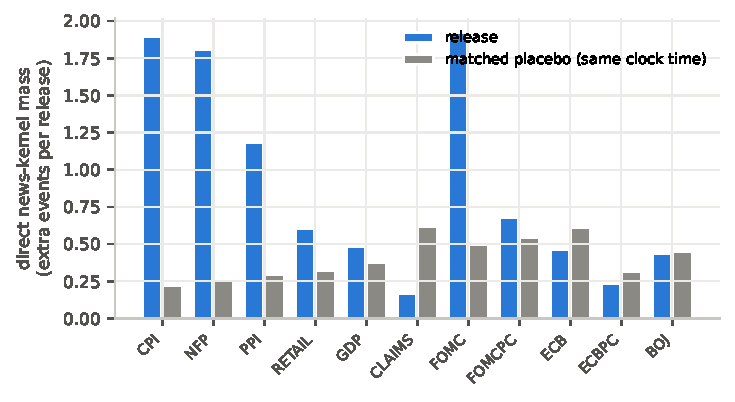
\includegraphics[width=0.72\linewidth]{figures/placebo_pooled.pdf}
\caption{Placebo test: direct news-kernel mass (expected extra events per release, all
assets) for each release type and for its matched placebo on release-free days.}\label{fig:placebo}
\end{figure}

\paragraph{Echo-corrected absorption.} For the releases that pass, the direct news kernel is
absorbed almost instantly (median $t_{50}$ of \tDirMed{}\,s), but echoes stretch the response:
half of the extra activity arrives within \tEchoLo--\tEchoHi{}\,s and ninety percent within
\tNinetyLo--\tNinetyHi{} minutes (Figure~\ref{fig:absorption}, Table~\ref{tab:absorption}).
The ``news half-life'' $\ln2/\beta$ therefore understates absorption time by one to two orders
of magnitude. Because signed surprises enter the news kernel separately by sign, the model also
gives price-discovery curves (Figure~\ref{fig:drift}, Table~\ref{tab:drift}); hotter inflation
lowers bitcoin and ether, cooler inflation lifts them.

\begin{figure}[!htbp]\centering
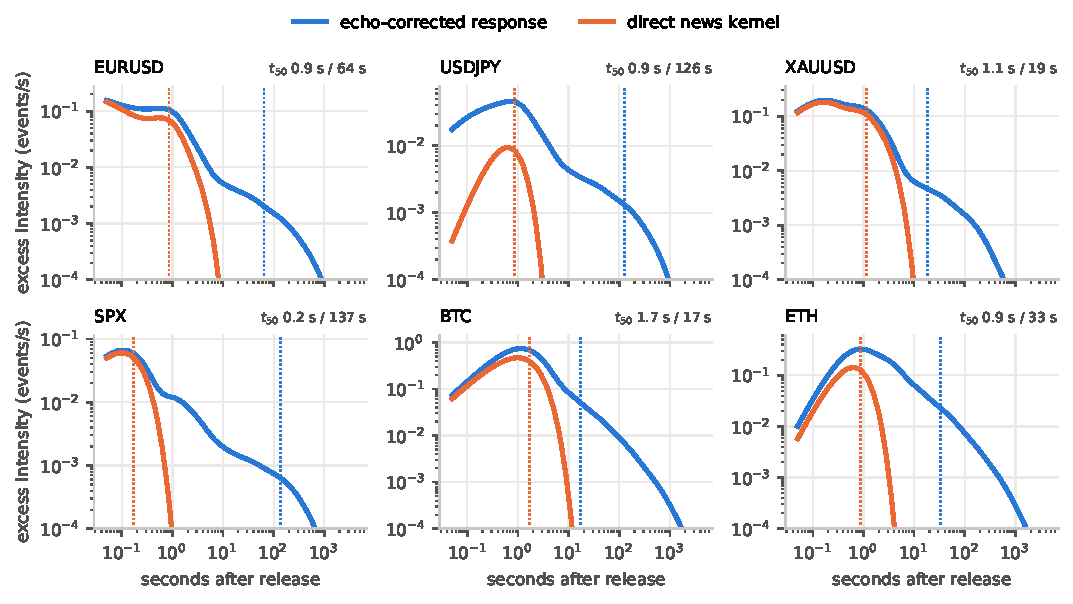
\includegraphics[width=\linewidth]{figures/absorption_CPI_pooled.pdf}
\caption{Echo-corrected response to a CPI release (blue) versus the direct news kernel
(orange), per asset; dotted lines mark $t_{50}$.}\label{fig:absorption}
\end{figure}

\begin{table}[!htbp]\centering\small
\caption{Echo-corrected absorption by release and asset: $t_{50}$ in seconds / $t_{90}$ in
minutes. $^\ast$Release types that do not exceed their placebo by 50\%.}\label{tab:absorption}
\setlength{\tabcolsep}{4pt}
\begin{tabular}{lcccccc}
\toprule
Release & EURUSD & USDJPY & Gold & S\&P 500 & BTC & ETH \\
\midrule
CPI & 64 / 9.1 & 126 / 11.0 & 19 / 4.8 & 137 / 11.0 & 17 / 6.1 & 33 / 7.8 \\
NFP & 94 / 10.1 & 109 / 10.7 & 16 / 5.2 & 80 / 8.8 & 27 / 7.5 & 24 / 7.3 \\
PPI & 120 / 10.8 & 94 / 10.3 & 40 / 6.4 & 79 / 8.6 & 23 / 7.2 & 39 / 8.7 \\
FOMC & 89 / 10.1 & 76 / 9.8 & 82 / 9.0 & 77 / 8.9 & 41 / 9.2 & 36 / 9.1 \\
Retail & 59 / 9.1 & 77 / 9.8 & 87 / 9.2 & 114 / 10.4 & 26 / 7.6 & 26 / 7.8 \\
\midrule
GDP$^\ast$ & 95 / 10.0 & 81 / 9.6 & 26 / 5.1 & 145 / 11.2 & 27 / 7.3 & 27 / 7.5 \\
FOMC press conf.$^\ast$ & 88 / 10.0 & 111 / 10.9 & 60 / 8.1 & 59 / 8.0 & 45 / 9.5 & 52 / 10.0 \\
Claims$^\ast$ & 124 / 11.0 & 56 / 9.1 & 87 / 9.3 & 81 / 9.1 & 36 / 9.0 & 40 / 9.4 \\
ECB$^\ast$ & 61 / 9.2 & 73 / 9.6 & 88 / 9.0 & 123 / 10.8 & 37 / 9.2 & 42 / 9.6 \\
ECB press conf.$^\ast$ & 137 / 11.3 & 90 / 10.2 & 38 / 6.5 & 63 / 8.2 & 25 / 7.3 & 32 / 8.0 \\
BoJ$^\ast$ & 93 / 10.2 & 80 / 9.9 & 45 / 7.3 & 73 / 8.8 & 35 / 8.5 & 37 / 8.8 \\
\bottomrule
\end{tabular}
\end{table}

\begin{figure}[!htbp]\centering
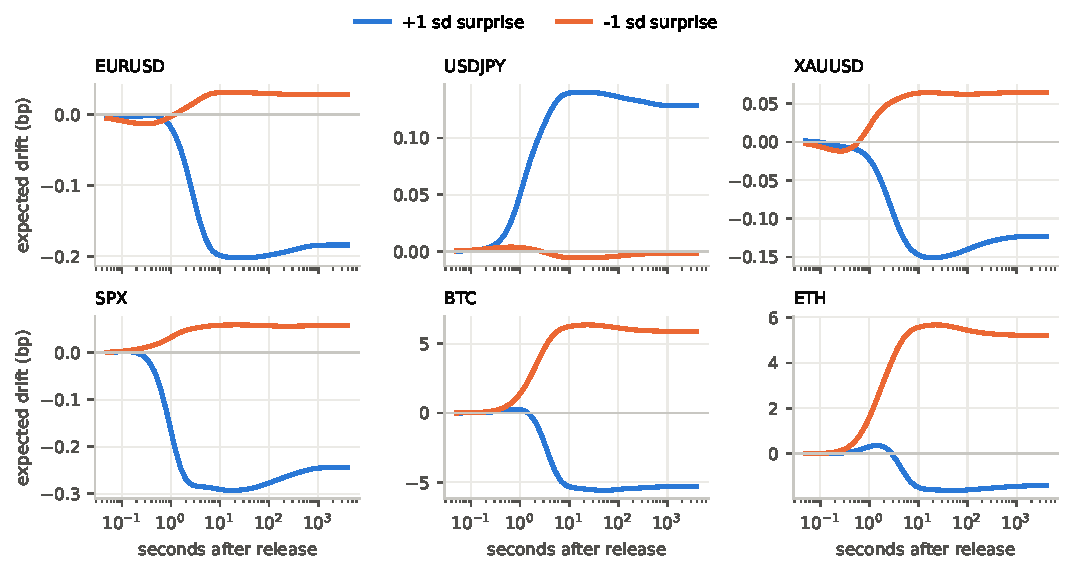
\includegraphics[width=\linewidth]{figures/drift_CPI_pooled.pdf}
\caption{Expected price-discovery curves after a $\pm1$ standard-deviation CPI surprise.}\label{fig:drift}
\end{figure}

\begin{table}[!htbp]\centering\small
\caption{Expected price drift (basis points, end of window) after a $+1$ standard-deviation
surprise. $^\ast$As in Table~\ref{tab:absorption}.}\label{tab:drift}
\setlength{\tabcolsep}{4pt}
\begin{tabular}{lcccccc}
\toprule
Release & EURUSD & USDJPY & Gold & S\&P 500 & BTC & ETH \\
\midrule
CPI & $-$0.2 & $+$0.1 & $-$0.1 & $-$0.2 & $-$5.3 & $-$1.4 \\
NFP & $-$0.1 & $+$0.1 & $+$0.1 & $+$0.2 & $-$0.3 & $-$1.5 \\
PPI & 0.0 & $+$0.1 & $-$0.2 & $-$0.3 & $-$2.4 & $-$2.1 \\
FOMC & 0.0 & $-$0.1 & $+$0.1 & $+$0.1 & $-$0.3 & $+$0.2 \\
Retail & $+$0.1 & $-$0.1 & $+$0.2 & 0.0 & $-$1.3 & $-$0.5 \\
\midrule
GDP$^\ast$ & $+$0.1 & $-$0.1 & $-$0.1 & 0.0 & $+$0.9 & $+$0.2 \\
FOMC press conf.$^\ast$ & 0.0 & 0.0 & 0.0 & $+$0.1 & 0.0 & $+$0.1 \\
Claims$^\ast$ & 0.0 & 0.0 & 0.0 & 0.0 & $+$0.4 & $+$0.6 \\
ECB$^\ast$ & 0.0 & 0.0 & 0.0 & 0.0 & $-$0.1 & $-$0.1 \\
ECB press conf.$^\ast$ & 0.0 & 0.0 & 0.0 & 0.0 & $-$0.3 & $-$0.3 \\
BoJ$^\ast$ & 0.0 & 0.0 & 0.0 & 0.0 & $-$0.1 & $+$0.3 \\
\bottomrule
\end{tabular}
\end{table}

\paragraph{Goodness of fit.} Time-rescaled residuals \citep{brown2002time} have
Kolmogorov--Smirnov statistics of at most \ksMax{} against Exp(1); the per-window
excess-dispersion test rejects in \edLo--\edHi\% of windows, compared with 42\% (power-law
kernel) and 93\% (double exponential) reported for FX data by \citet{rambaldi2015modeling}.

\paragraph{Forecasting the post-release burst.} On the \nTestReleases{} releases of 2025--2026,
an MSX model fitted on 2022--2024 forecasts the number of $\delta$-crossings in the first 1, 5
and 15 minutes in closed form (Table~\ref{tab:track-d}). It improves on same-type climatology
at every horizon but is beaten by the \bestActivityModel{} and HAR regressions, which are fitted
directly to this target; we report this negative result as is. For the direction of the move
the structural model is informative: the correlation between its forecast and the realised
one-minute drift is \driftCorrOursOne{}, against \driftCorrBaseOne{} for the best baseline.

\begin{table}[!htbp]\centering\small
\caption{Post-release activity forecasts on the \nTestReleases{} test releases (mean over
assets; lower is better). Bold: best; underlined: second best; shaded: our model.}\label{tab:track-d}
\setlength{\tabcolsep}{5pt}
\begin{tabular}{lrrrrrr}
\toprule
& \multicolumn{3}{c}{RMSE of $\log(1+N)$} & \multicolumn{3}{c}{QLIKE of realised variance} \\
\cmidrule(lr){2-4}\cmidrule(lr){5-7}
Method & 1 min & 5 min & 15 min & 1 min & 5 min & 15 min \\
\midrule
Climatology & 1.440 & 1.308 & 1.199 & \textbf{1.263} & 0.916 & 0.701 \\
Event-study OLS & \textbf{1.140} & \textbf{0.925} & \textbf{0.776} & 2.552 & \textbf{0.580} & \textbf{0.372} \\
HAR & \underline{1.217} & \underline{0.985} & \underline{0.820} & \underline{1.467} & \underline{0.762} & \underline{0.468} \\
\rowcolor{oursbg} MSX closed form & 1.322 & 1.049 & 0.955 & 2.913 & 1.036 & 0.518 \\
\bottomrule
\end{tabular}
\end{table}

\section{Discussion and limitations}\label{sec:discussion}

Making every kernel a nonnegative combination of phase-type densities turns Hawkes
estimation into a certified convex problem and turns responses to shocks into matrix
exponentials; adding a neural history encoder and a defective hyper-Erlang renewal channel to
the same state space gives a model whose likelihood stays exact and which is competitive with,
and on order books and Retweet better than, the strongest neural temporal point processes.
Three lessons stand out. First, absorption speed is not a property of the news kernel: echoes
lengthen it by one to two orders of magnitude, and the correction is available in closed form.
Second, falsification matters: two of our specifications produced plausible-looking news
effects that the placebo test exposed as artefacts. Third, benchmark comparisons must check
that every model scores the same observed data---a clamp inside one implementation was enough
to reverse a ranking.

\paragraph{Limitations.} Expectations for payrolls, claims, PPI and retail sales are
statistical rather than survey-based, and the FX feed has a gap in the first half of 2023. The
order-book evaluation uses the public LOBSTER samples (one trading day per stock). Neural
baselines on order books were trained with reduced batch sizes on an 8\,GB GPU, and on the
public benchmarks we compare against published numbers, validated by one re-run. On Retweet the
EPT-X budget was 25 epochs with the validation likelihood still rising, so the reported margin
is if anything conservative. EPT-X does not reach the best published likelihood on Taxi, where
the gap lies in mark prediction, or on Amazon, where it lies in the timing density; and the
MSX forecasts of post-release activity are beaten by regressions fitted to that target.


\subsubsection*{Broader Impact Statement}
This work models market event streams with public or licensable data and makes no use of
personal data. Better models of how quickly prices absorb public information can inform market
monitoring and the timing of disclosures, and exact likelihoods make benchmark comparisons more
reliable. Faster or more accurate event forecasts could also be used in trading; the methods
described are standard statistical tools and do not by themselves confer an informational
advantage. We release code and patches so that the reported numbers, including the corrected
baseline, can be reproduced.


\subsubsection*{Reproducibility Statement}
All result tables and every number quoted in the text are generated by scripts from the logged
outputs of the experiments; the \codename{} contains the models, the experiment and
table scripts, the EasyTPP patches (tie handling and the IntensityFree clamp), configuration
files and unit tests (exact compensators against numerical quadrature, causality of the
encoders, nesting of EPT-X in EPT). Public datasets are used through their standard splits;
the market data are licensed from their providers and are not redistributed.

\bibliography{refs}
\bibliographystyle{tmlr}

\appendix
\section{Proofs}\label{app:proofs}

\begin{proof}[Proof of Proposition~\ref{prop:gap}]
Fenchel's inequality $\log u\le vu-1-\log v$ for $u,v>0$, applied to $u=\lambda_n$ with
$v=v_n$, gives $\sum_n\log\lambda_n\le\bm\theta^\top X^\top\bm v-N-\sum_n\log v_n$. If
$X^\top\bm v\le\bm\Phi+\bm\gamma$ then $\bm\theta^\top X^\top\bm v\le\bm\theta^\top(\bm\Phi+\bm\gamma)$
for every $\bm\theta\ge0$, hence $\ell(\bm\theta)\le D(\bm v):=-N-\sum_n\log v_n$ for every
feasible $\bm\theta$, including the maximiser. The choice $v_n=1/(s\lambda_n)$ with $s$ as
stated is dual feasible and gives $D(\bm v)-\ell(\bm\theta)=N\log s+\bm\theta^\top(\bm\Phi+\bm\gamma)-N$.
At a KKT point $s=1$ and $\bm\theta^\top(\bm\Phi+\bm\gamma)=\sum_n\bm\theta^\top\bm x_n/\lambda_n=N$,
so both terms vanish.
\end{proof}

\section{Specification history of the application}\label{app:history}
We report the specifications that failed the built-in falsification test, because the final
specification was chosen by them rather than by the results we hoped for.

\paragraph{Version 1.} News kernels with time scales up to 30 minutes and Erlang order 3, a
constant baseline per window, time-of-day hats in UTC, and tied events (a trade sweeping
several $\delta$ levels produced several events with the same timestamp). The single placebo
type absorbed \vOnePlacebo{} extra events per pseudo-release, comparable to real releases,
and crypto residuals had Kolmogorov--Smirnov statistics up to \vOneKSmax. News kernels longer
than the post-release window acted as trend absorbers, and ties violated orderliness.

\paragraph{Version 2.} One event per timestamp with a size mark, news kernels restricted to
0.1--300\,s, a per-window linear baseline and New-York-time seasonality. The placebo mass fell
to \vTwoPlacebo{}, but remained significant; placebo mass appeared at every release slot,
which ruled out unmodelled 08:30 releases as the whole explanation.

\paragraph{Version 3 (final).} Placebo days also avoid sixteen second-tier US releases, and
nonnegative news kernels carry an exposure-weighted $\ell_1$ penalty chosen by held-out
profile likelihood (Table~\ref{tab:l1}); without it, release and placebo masses are equally
inflated by boundary bias. The held-out likelihood peaks at $\ell_1=\lOneSelected$, where
release and placebo masses separate.

\begin{table}[!htbp]\centering\small
\caption{Selection of the news-kernel penalty on held-out 2024 windows (profile
log-likelihood relative to the best level).}\label{tab:l1}
\begin{tabular}{cccc}
\toprule
$\ell_1$ level & held-out LL (rel.) & mean release mass & mean placebo mass \\
\midrule
0.2 & {-93.7} & 10.79 & 6.23 \\
0.4 & {-27.1} & 5.20 & 2.89 \\
0.8 & \textbf{0.0} & 1.81 & 1.03 \\
1.6 & {-20.5} & 0.44 & 0.37 \\
\bottomrule
\end{tabular}
\end{table}

\section{Synthetic recovery: all metrics}\label{app:synthetic}
\begin{table}[!htbp]\centering\scriptsize
\caption{Synthetic recovery, all metrics (mean $\pm$ s.d.\ over five seeds): relative
branching-matrix error, spectral-radius error, kernel $L^1$ error, held-out deficit dLL
($10^{-3}$ nats/event) and edge AUC. AUC measures how well absent and present edges are
separated, so it is defined only for scenarios whose true graph has absent edges (S4, S5);
``n/a'' marks S1--S3, whose graphs are complete. ``--'' marks a metric the method does not
produce (NPHC estimates only the branching matrix, not kernels or a likelihood); rows absent
for a scenario are fits that failed to converge.}\label{tab:track-a-full}
\resizebox{\linewidth}{!}{\begin{tabular}{llccccc}
\toprule
Scenario & Method & $G$ err. & $\rho$ err. & kernel $L^1$ & dLL ($10^{-3}$) & AUC \\
\midrule
S1-exp & MSX-auto (ours) & 0.054 $\pm$ 0.032 & 0.020 $\pm$ 0.018 & 0.093 & 0.24 $\pm$ 0.12 & -- \\
 & MSX (ours) & 0.056 $\pm$ 0.032 & 0.019 $\pm$ 0.018 & 0.092 & 0.23 $\pm$ 0.12 & -- \\
 & MSX-R4 (ours, fixed Erlang-4) & 0.056 $\pm$ 0.035 & 0.023 $\pm$ 0.018 & 0.105 & 0.28 $\pm$ 0.15 & -- \\
 & MSX-exp (ablation: no Erlang) & 0.055 $\pm$ 0.025 & 0.026 $\pm$ 0.015 & 0.157 & 0.91 $\pm$ 0.13 & -- \\
 & ExpKern(MLE, best decay) & 0.018 $\pm$ 0.007 & 0.005 $\pm$ 0.003 & 0.018 & \textbf{0.05 $\pm$ 0.05} & -- \\
 & SumExpKern(MLE, AGD) & 0.065 $\pm$ 0.022 & 0.030 $\pm$ 0.013 & 0.165 & 0.92 $\pm$ 0.13 & -- \\
 & ADM4 & 0.018 $\pm$ 0.007 & 0.005 $\pm$ 0.003 & 0.018 & 0.05 $\pm$ 0.05 & -- \\
 & EM(nonparam) & 0.035 $\pm$ 0.015 & 0.017 $\pm$ 0.007 & 0.173 & 1.02 $\pm$ 0.07 & -- \\
 & NPHC(cumulants) & 0.247 $\pm$ 0.087 & 0.032 $\pm$ 0.024 & -- & -- & -- \\
 & ConditionalLaw & 0.120 $\pm$ 0.054 & 0.017 $\pm$ 0.016 & 0.193 & 2.84 $\pm$ 1.03 & -- \\
\midrule
S2-powerlaw & MSX-auto (ours) & 0.064 $\pm$ 0.029 & 0.037 $\pm$ 0.029 & 0.108 & 0.33 $\pm$ 0.13 & -- \\
 & MSX (ours) & 0.057 $\pm$ 0.021 & 0.015 $\pm$ 0.010 & 0.114 & 0.32 $\pm$ 0.12 & -- \\
 & MSX-R4 (ours, fixed Erlang-4) & 0.062 $\pm$ 0.014 & 0.016 $\pm$ 0.006 & 0.131 & 0.45 $\pm$ 0.10 & -- \\
 & MSX-exp (ablation: no Erlang) & 0.054 $\pm$ 0.022 & 0.014 $\pm$ 0.010 & 0.097 & 0.19 $\pm$ 0.11 & -- \\
 & ExpKern(MLE, best decay) & 0.299 $\pm$ 0.011 & 0.219 $\pm$ 0.007 & 0.465 & 26.05 $\pm$ 0.50 & -- \\
 & SumExpKern(MLE, AGD) & 0.057 $\pm$ 0.012 & 0.016 $\pm$ 0.007 & 0.094 & \textbf{0.18 $\pm$ 0.12} & -- \\
 & ADM4 & 0.299 $\pm$ 0.011 & 0.219 $\pm$ 0.007 & 0.465 & 26.05 $\pm$ 0.50 & -- \\
 & EM(nonparam) & 0.057 $\pm$ 0.014 & 0.037 $\pm$ 0.008 & 0.188 & 1.73 $\pm$ 0.21 & -- \\
 & NPHC(cumulants) & 0.153 $\pm$ 0.154 & 0.041 $\pm$ 0.047 & -- & -- & -- \\
 & ConditionalLaw & 0.102 $\pm$ 0.067 & 0.029 $\pm$ 0.019 & 0.291 & 4.91 $\pm$ 0.59 & -- \\
\midrule
S3-hump & MSX-auto (ours) & 0.032 $\pm$ 0.016 & 0.016 $\pm$ 0.007 & 0.080 & \textbf{0.30 $\pm$ 0.13} & -- \\
 & MSX (ours) & 0.069 $\pm$ 0.009 & 0.037 $\pm$ 0.004 & 0.347 & 5.90 $\pm$ 0.36 & -- \\
 & MSX-R4 (ours, fixed Erlang-4) & 0.038 $\pm$ 0.010 & 0.017 $\pm$ 0.005 & 0.074 & 0.31 $\pm$ 0.15 & -- \\
 & MSX-exp (ablation: no Erlang) & 0.034 $\pm$ 0.009 & 0.015 $\pm$ 0.004 & 0.416 & 11.51 $\pm$ 0.46 & -- \\
 & ExpKern(MLE, best decay) & 0.166 $\pm$ 0.008 & 0.053 $\pm$ 0.004 & 0.801 & 101.47 $\pm$ 1.81 & -- \\
 & SumExpKern(MLE, AGD) & 0.038 $\pm$ 0.011 & 0.018 $\pm$ 0.005 & 0.419 & 11.51 $\pm$ 0.46 & -- \\
 & ADM4 & 0.166 $\pm$ 0.008 & 0.053 $\pm$ 0.004 & 0.801 & 101.47 $\pm$ 1.81 & -- \\
 & EM(nonparam) & 0.024 $\pm$ 0.011 & 0.010 $\pm$ 0.004 & 0.187 & 2.24 $\pm$ 0.12 & -- \\
 & NPHC(cumulants) & 0.240 $\pm$ 0.096 & 0.045 $\pm$ 0.048 & -- & -- & -- \\
 & ConditionalLaw & 0.149 $\pm$ 0.062 & 0.017 $\pm$ 0.010 & 0.319 & 10.66 $\pm$ 2.13 & -- \\
\midrule
S4-multiscale & MSX-auto (ours) & 0.084 $\pm$ 0.014 & 0.016 $\pm$ 0.006 & 0.128 & \textbf{0.32 $\pm$ 0.08} & 1.000 \\
 & MSX (ours) & 0.093 $\pm$ 0.015 & 0.021 $\pm$ 0.005 & 0.173 & 0.54 $\pm$ 0.12 & 1.000 \\
 & MSX-R4 (ours, fixed Erlang-4) & 0.101 $\pm$ 0.019 & 0.027 $\pm$ 0.007 & 0.207 & 0.70 $\pm$ 0.11 & 1.000 \\
 & MSX-exp (ablation: no Erlang) & 0.084 $\pm$ 0.014 & 0.016 $\pm$ 0.006 & 0.128 & \textbf{0.32 $\pm$ 0.08} & 1.000 \\
 & ExpKern(MLE, best decay) & 0.173 $\pm$ 0.041 & 0.095 $\pm$ 0.025 & 1.635 & 711.28 $\pm$ 53.09 & 1.000 \\
 & ADM4 & 0.399 $\pm$ 0.003 & 0.255 $\pm$ 0.001 & 0.410 & 3.13 $\pm$ 0.25 & 1.000 \\
 & EM(nonparam) & 0.153 $\pm$ 0.012 & 0.045 $\pm$ 0.010 & 0.358 & 4.55 $\pm$ 0.29 & 1.000 \\
 & NPHC(cumulants) & 1.030 $\pm$ 0.304 & 0.211 $\pm$ 0.186 & -- & -- & 0.588 \\
 & ConditionalLaw & 0.464 $\pm$ 0.286 & 0.139 $\pm$ 0.050 & 1.059 & 114.94 $\pm$ 1.20 & 0.831 \\
\midrule
S5-network10 & MSX-auto (ours) & 0.045 $\pm$ 0.004 & 0.015 $\pm$ 0.005 & 0.079 & \textbf{0.74 $\pm$ 0.10} & 1.000 \\
 & MSX (ours) & 0.111 $\pm$ 0.013 & 0.040 $\pm$ 0.013 & 0.180 & 1.19 $\pm$ 0.07 & 1.000 \\
 & MSX-R4 (ours, fixed Erlang-4) & 0.122 $\pm$ 0.008 & 0.051 $\pm$ 0.013 & 0.218 & 1.63 $\pm$ 0.09 & 1.000 \\
 & MSX-exp (ablation: no Erlang) & 0.099 $\pm$ 0.014 & 0.030 $\pm$ 0.014 & 0.145 & 0.82 $\pm$ 0.08 & 1.000 \\
 & ExpKern(MLE, best decay) & 0.337 $\pm$ 0.153 & 0.103 $\pm$ 0.032 & 1.302 & 426.80 $\pm$ 368.57 & 0.977 \\
 & ADM4 & 0.167 $\pm$ 0.003 & 0.096 $\pm$ 0.003 & 0.319 & 26.51 $\pm$ 0.29 & 1.000 \\
 & EM(nonparam) & 0.085 $\pm$ 0.008 & 0.045 $\pm$ 0.008 & 0.280 & 5.23 $\pm$ 0.25 & 1.000 \\
 & NPHC(cumulants) & 1.348 $\pm$ 0.477 & 0.520 $\pm$ 0.372 & -- & -- & 0.672 \\
 & ConditionalLaw & 0.461 $\pm$ 0.047 & 0.037 $\pm$ 0.026 & 0.641 & 78.64 $\pm$ 4.79 & 0.950 \\
\bottomrule
\end{tabular}}
\end{table}

\section{Experimental details}\label{app:details}

\paragraph{MSX.} Endogenous dictionary: 10 rates from 5\,ms to 600\,s, Erlang order 2;
exogenous: 8 rates from 0.1 to 300\,s, order 3, marks $(1,z^+,z^-)$; anticipation: 4 rates
from 10 to 300\,s; 96 time-of-day hats; per-window linear baseline. On public and order-book
benchmarks MSX uses a shared baseline and a 12-rate grid spanning the 1st percentile to five
times the 99.9th percentile of training gaps, and MSX-auto selects the Erlang order in $\{1,2,3,4\}$ and the $\ell_1$ level
in $\{0,0.01,0.05\}$ on the validation split.

\paragraph{EPT and EPT-X.} GRU with 64 units; 4 latent channels of 8 learnable rates; Erlang
phases selected on validation from $\{2,4\}$ (with hidden size $\{64,128\}$) on Taxi, Taobao and
StackOverflow; Hawkes backbone with 10 rates and 2 phases; AdamW with learning rate $10^{-2}$,
1\% linear warm-up and cosine decay, gradient clipping at 1, batch size 64 (halved
automatically on out-of-memory), early stopping on validation likelihood with patience 40 and
a 300-epoch budget (25 epochs on Retweet, batch 32). The renewal channel uses 24 log-spaced
mean gaps from half the 0.1\% to five times the 99.9\% quantile of training gaps with orders
$\{1,4,16\}$. Selected on validation, the LOBSTER streams and Amazon add orders up to 1024 and a
history-dependent shift, and Amazon uses a finer grid (single-seed validation log-likelihood
0.604, 0.643, 0.653 and 0.649 with 24, 48, 96 and 192 scales; 96 is selected). Mark laws are initialised at empirical frequencies.

\paragraph{Baselines.} Neural baselines run in EasyTPP with the authors' configuration files;
classical Hawkes estimators use the \texttt{tick} library (positive-constrained
accelerated gradient descent, tolerance $10^{-10}$, decay grids matched to MSX). The IntensityFree clamp is made configurable by a
two-line patch included in the supplementary code.

\paragraph{Compute.} All experiments ran on one laptop with an 8\,GB GPU and a 28-core CPU;
CPU jobs were limited to four threads each. EPT-X runs on the CPU at a speed comparable to the
GPU, because its event recursion is sequential.


\end{document}
